\section{Including Hybrid Municipalities}
\label{app:including-hybrid}
\label{app:exclude-hybrid}

The main registry specifications use strict biometric registration as the treatment and exclude municipalities ever flagged as hybrid. This appendix repeats the Callaway--Sant'Anna event studies using a broader treatment definition that includes both strict and hybrid BVR municipalities. This is a lower-intensity specification: hybrid municipalities could have biometric updates before full enforcement, but voters were not yet subject to the same complete recadastramento requirement as in strict municipalities.

The hybrid-inclusive estimates preserve the same qualitative pattern as the strict-BVR estimates, but the impact effects are smaller. For the size of the electorate, the event-time $0$ estimate moves from about $-0.117$ log points in the strict sample to about $-0.068$ log points when hybrid municipalities are included. For electorate composition, the low-education share falls by about 5.1 percentage points and the high-education share rises by about 5.1 percentage points at impact, compared with about 8.9 and 9.0 percentage points in the strict sample. The attenuation is consistent with hybrid BVR being a partial or lower-compliance-cost version of the reform rather than a different mechanism.

\begin{figure}[p]
    \caption{Including Hybrid Municipalities: Electorate Size}
    \label{fig:appendix-size-including-hybrid}
    \centering
    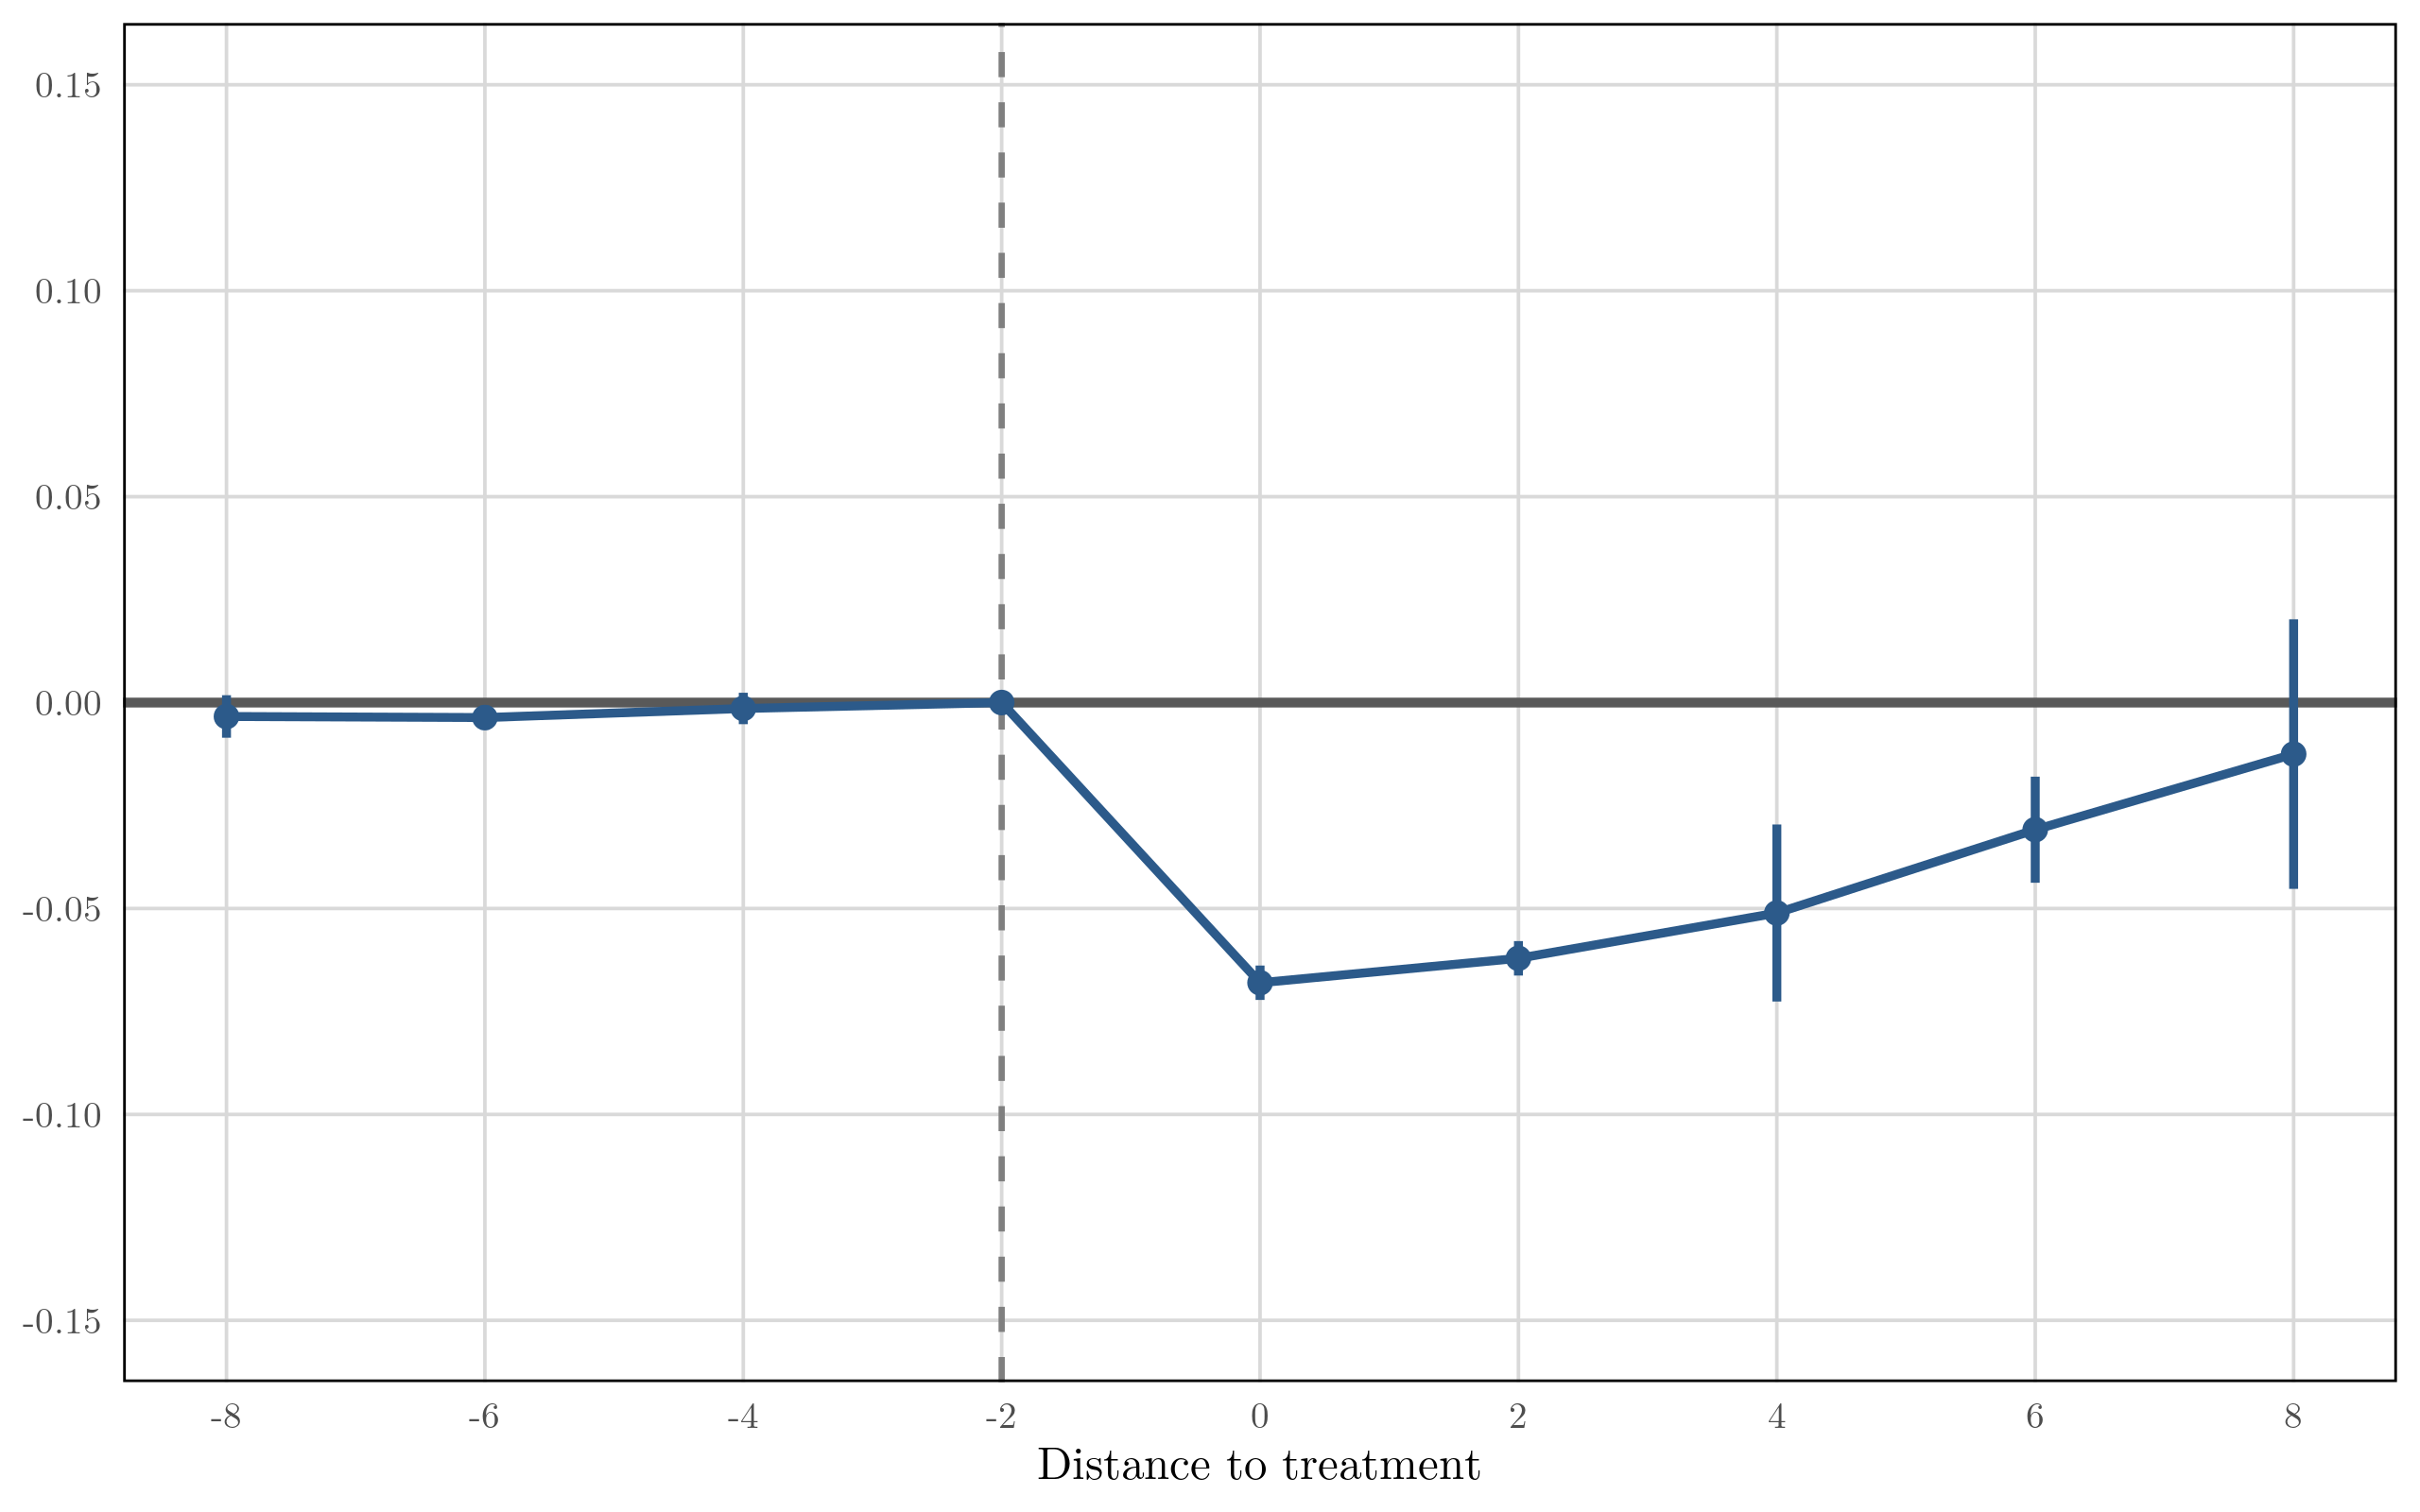
\includegraphics[width=0.72\textwidth]{../resources/regressions/bvr/log_num_voters/including_hybrid/callaway_santanna/event_study_plot.png}
    \vspace{0.75em}
    \begin{minipage}{\textwidth}
        {\footnotesize \textbf{Note:} The figure plots Callaway--Sant'Anna dynamic event-study estimates for the log number of registered voters after defining treatment as either strict or hybrid BVR. Never-treated municipalities are the control group. Event time $-2$ is the reference period and is shown at zero. Error bars report 95\% confidence intervals with standard errors clustered by municipality. \par}
    \end{minipage}
\end{figure}

\begin{figure}[p]
    \caption{Including Hybrid Municipalities: Education Composition}
    \label{fig:appendix-composition-including-hybrid}
    \centering
    \begin{subfigure}[b]{0.49\textwidth}
        \centering
        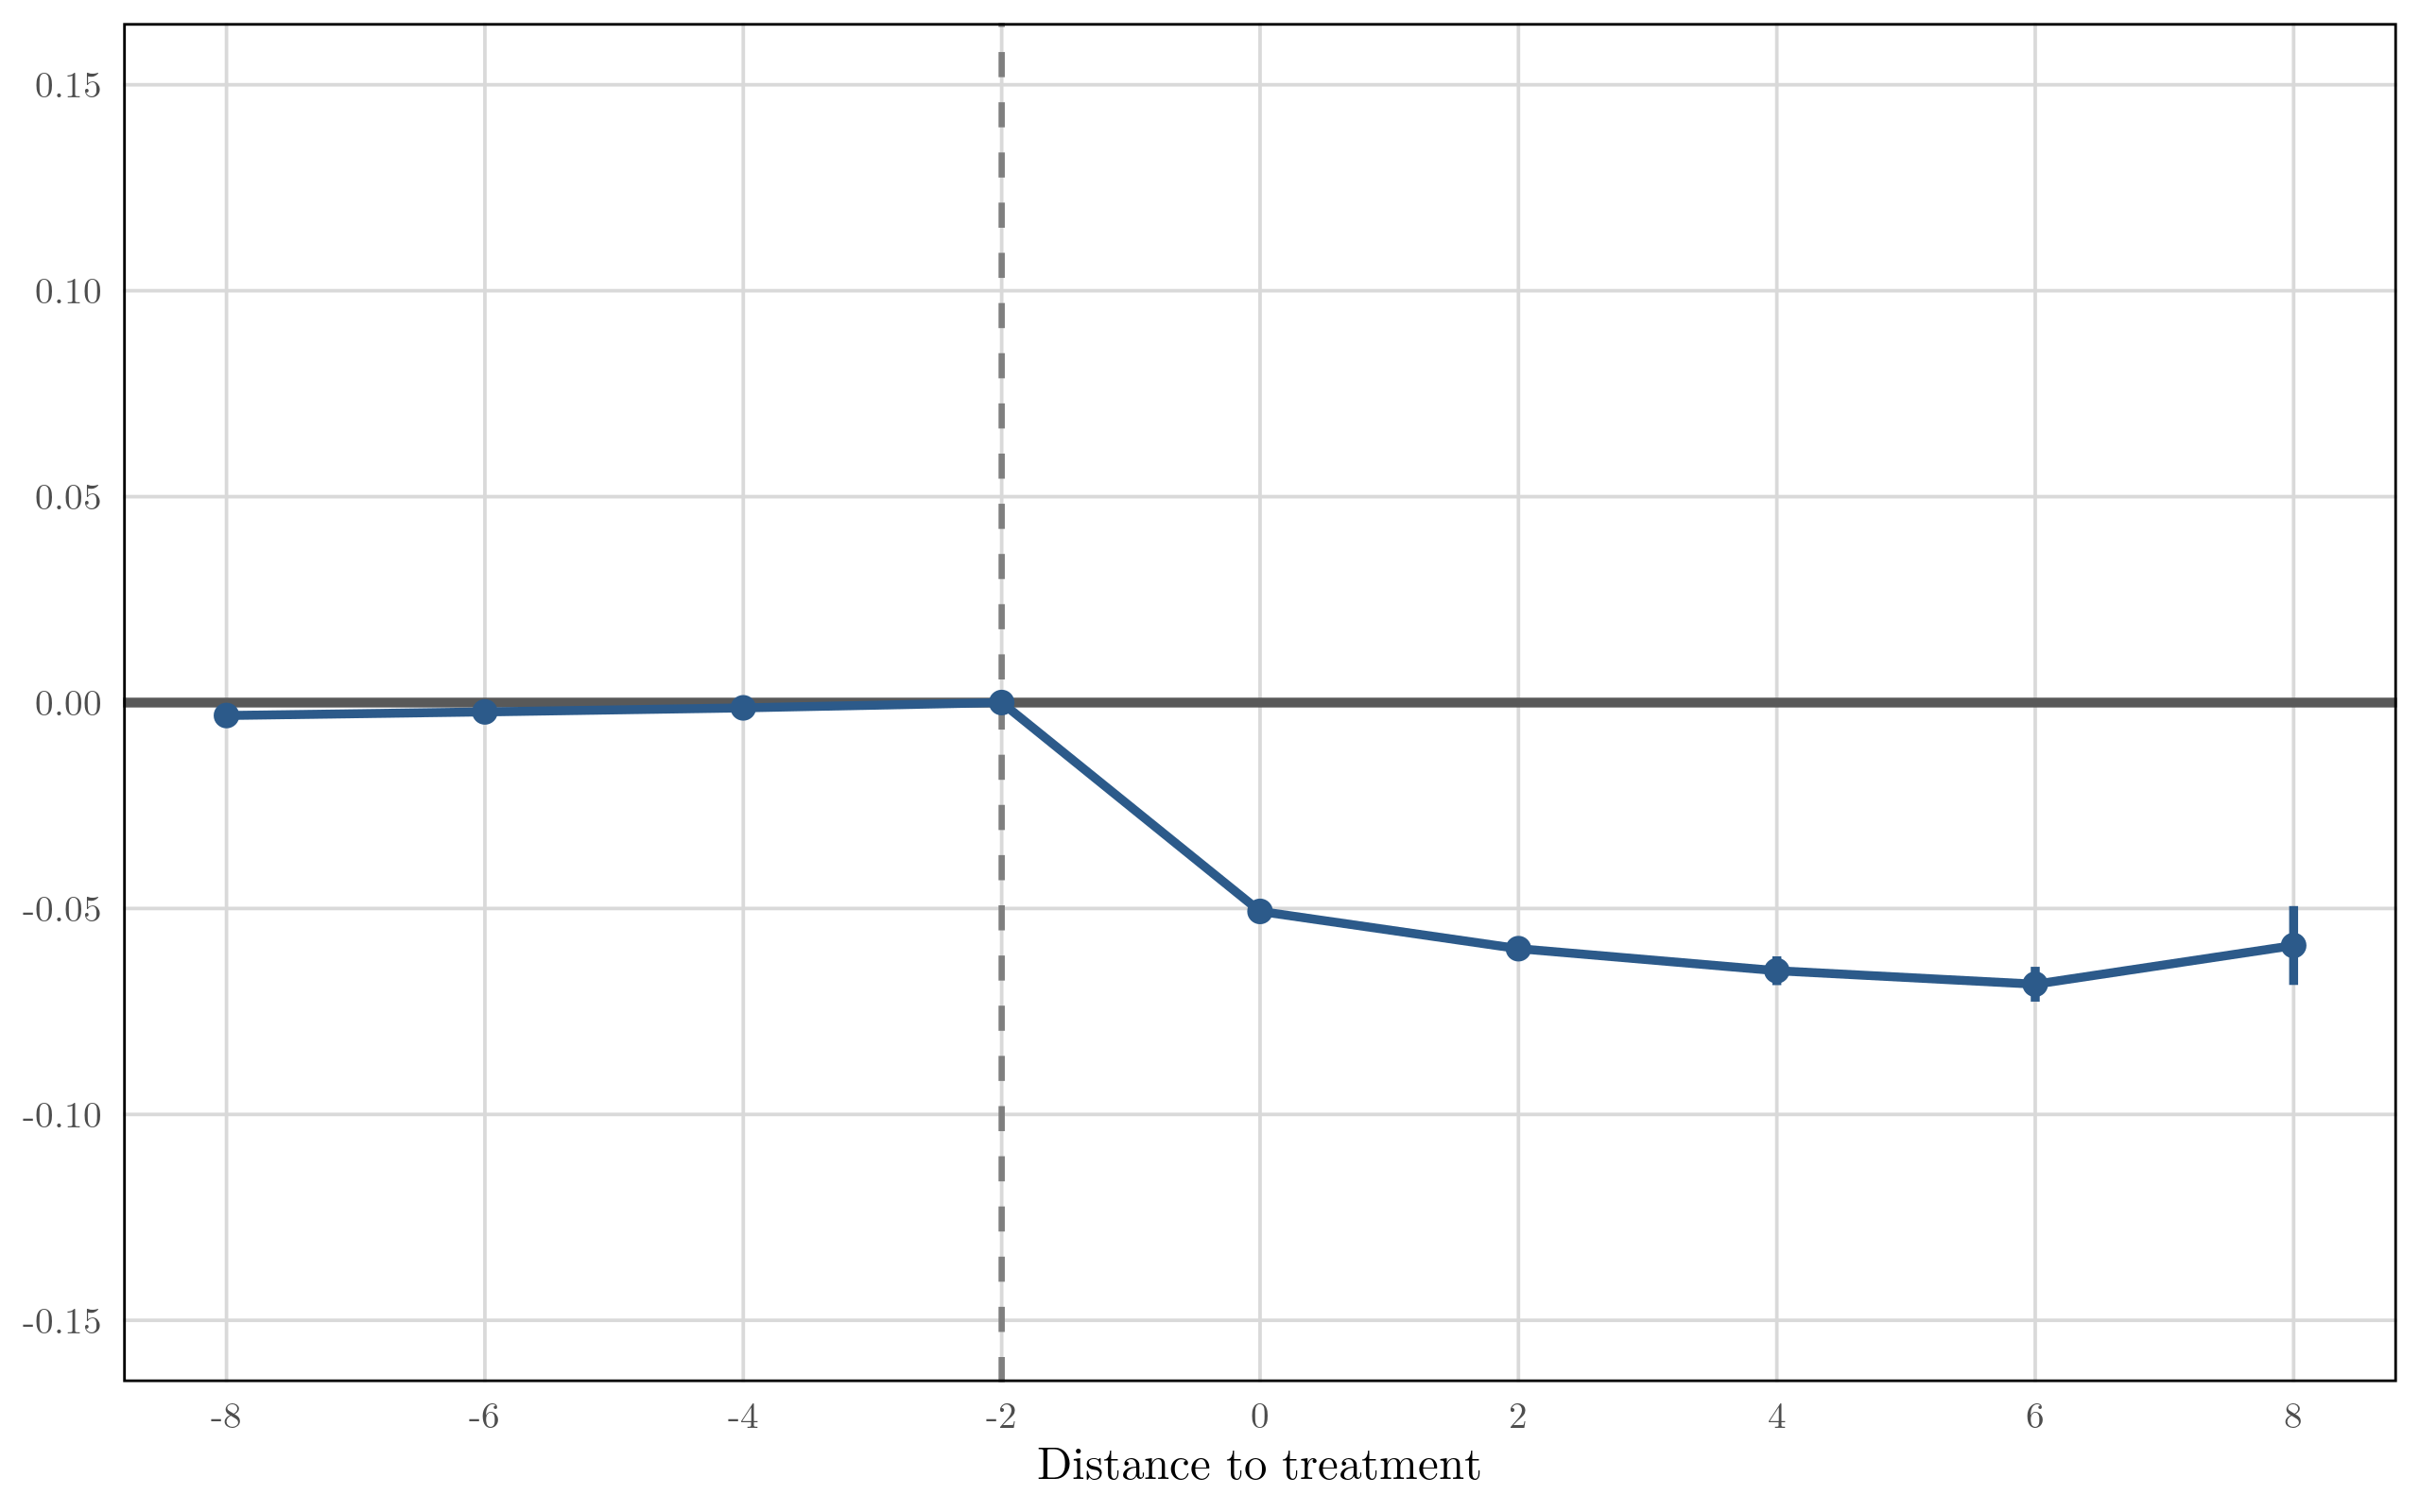
\includegraphics[width=\textwidth]{../resources/regressions/bvr/pct_voters_low_ed/including_hybrid/callaway_santanna/event_study_plot.png}
        \caption{Low-education share}
        \label{fig:appendix-low-education-including-hybrid}
    \end{subfigure}
    \hfill
    \begin{subfigure}[b]{0.49\textwidth}
        \centering
        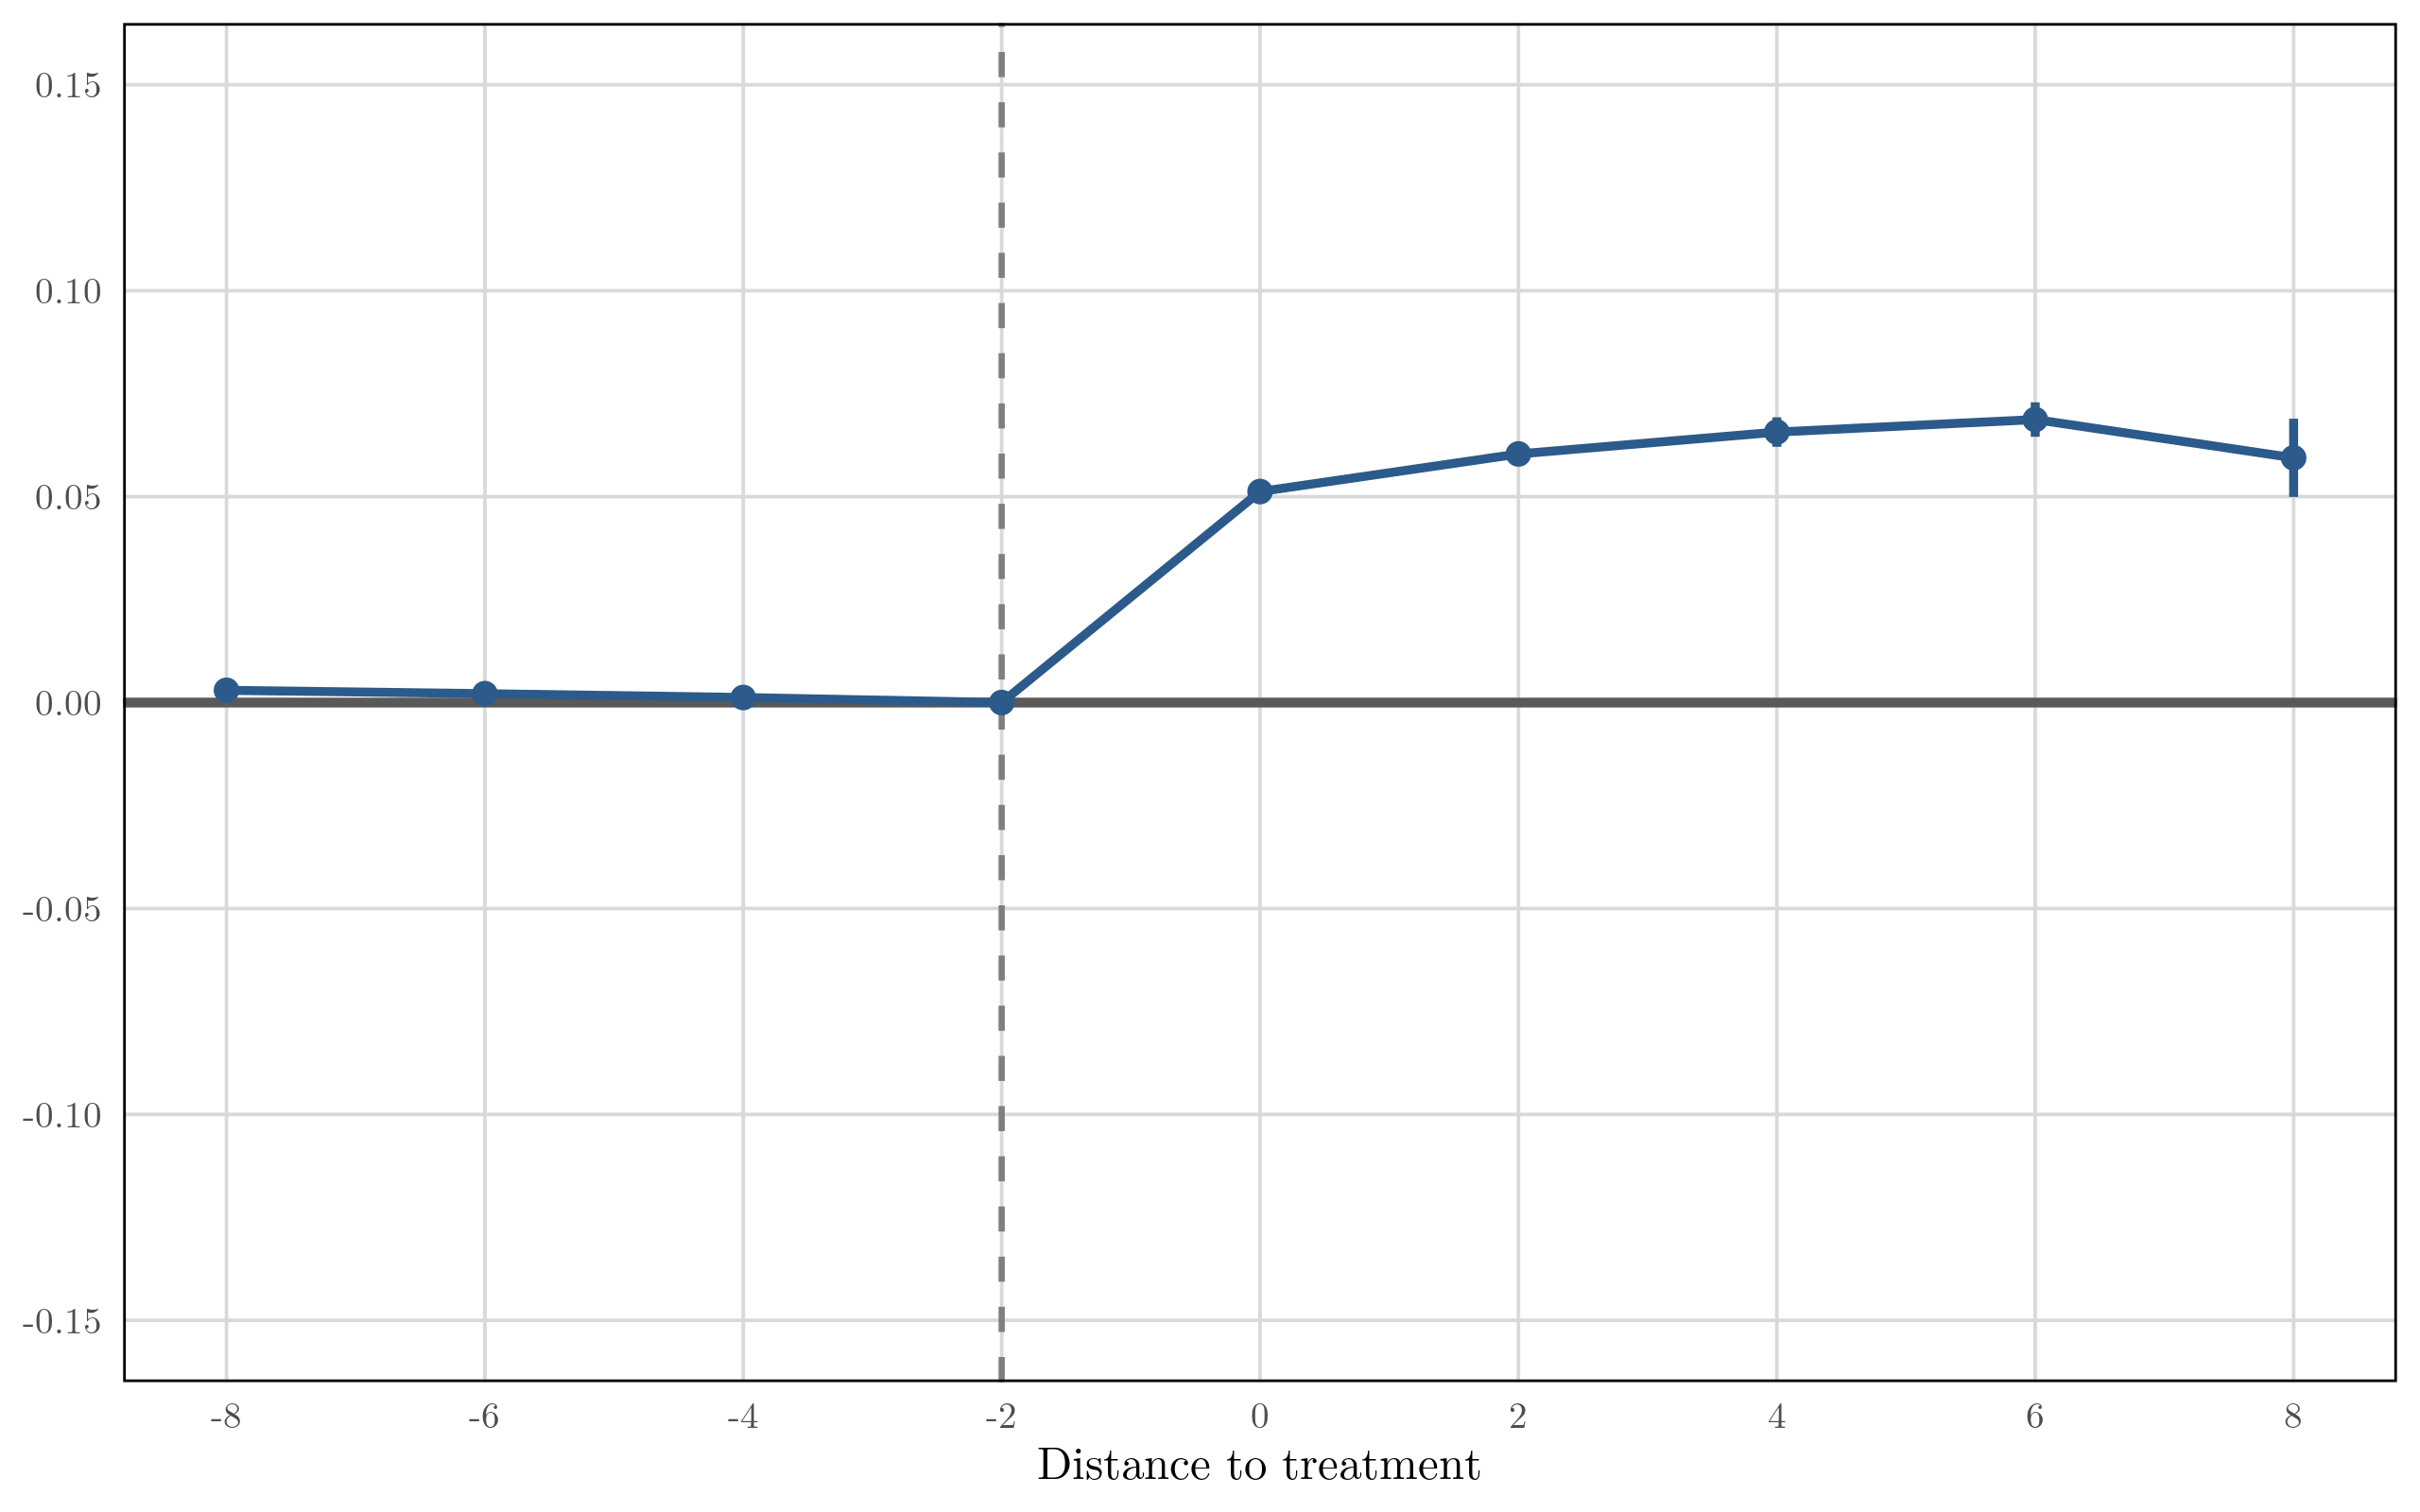
\includegraphics[width=\textwidth]{../resources/regressions/bvr/pct_voters_high_ed/including_hybrid/callaway_santanna/event_study_plot.png}
        \caption{High-education share}
        \label{fig:appendix-high-education-including-hybrid}
    \end{subfigure}
    \vspace{0.75em}
    \begin{minipage}{\textwidth}
        {\footnotesize \textbf{Note:} Each panel plots Callaway--Sant'Anna dynamic event-study estimates after defining treatment as either strict or hybrid BVR. Panel (a) uses the share of registered voters with schooling below completed secondary education as the outcome. Panel (b) uses the share with incomplete secondary schooling or more. Never-treated municipalities are the control group. Event time $-2$ is the reference period and is shown at zero. Error bars report 95\% confidence intervals with standard errors clustered by municipality. \par}
    \end{minipage}
\end{figure}

\begin{figure}[p]
    \caption{Including Hybrid Municipalities: Electorate Size Across Estimators}
    \label{fig:appendix-size-including-hybrid-estimator-comparison}
    \centering
    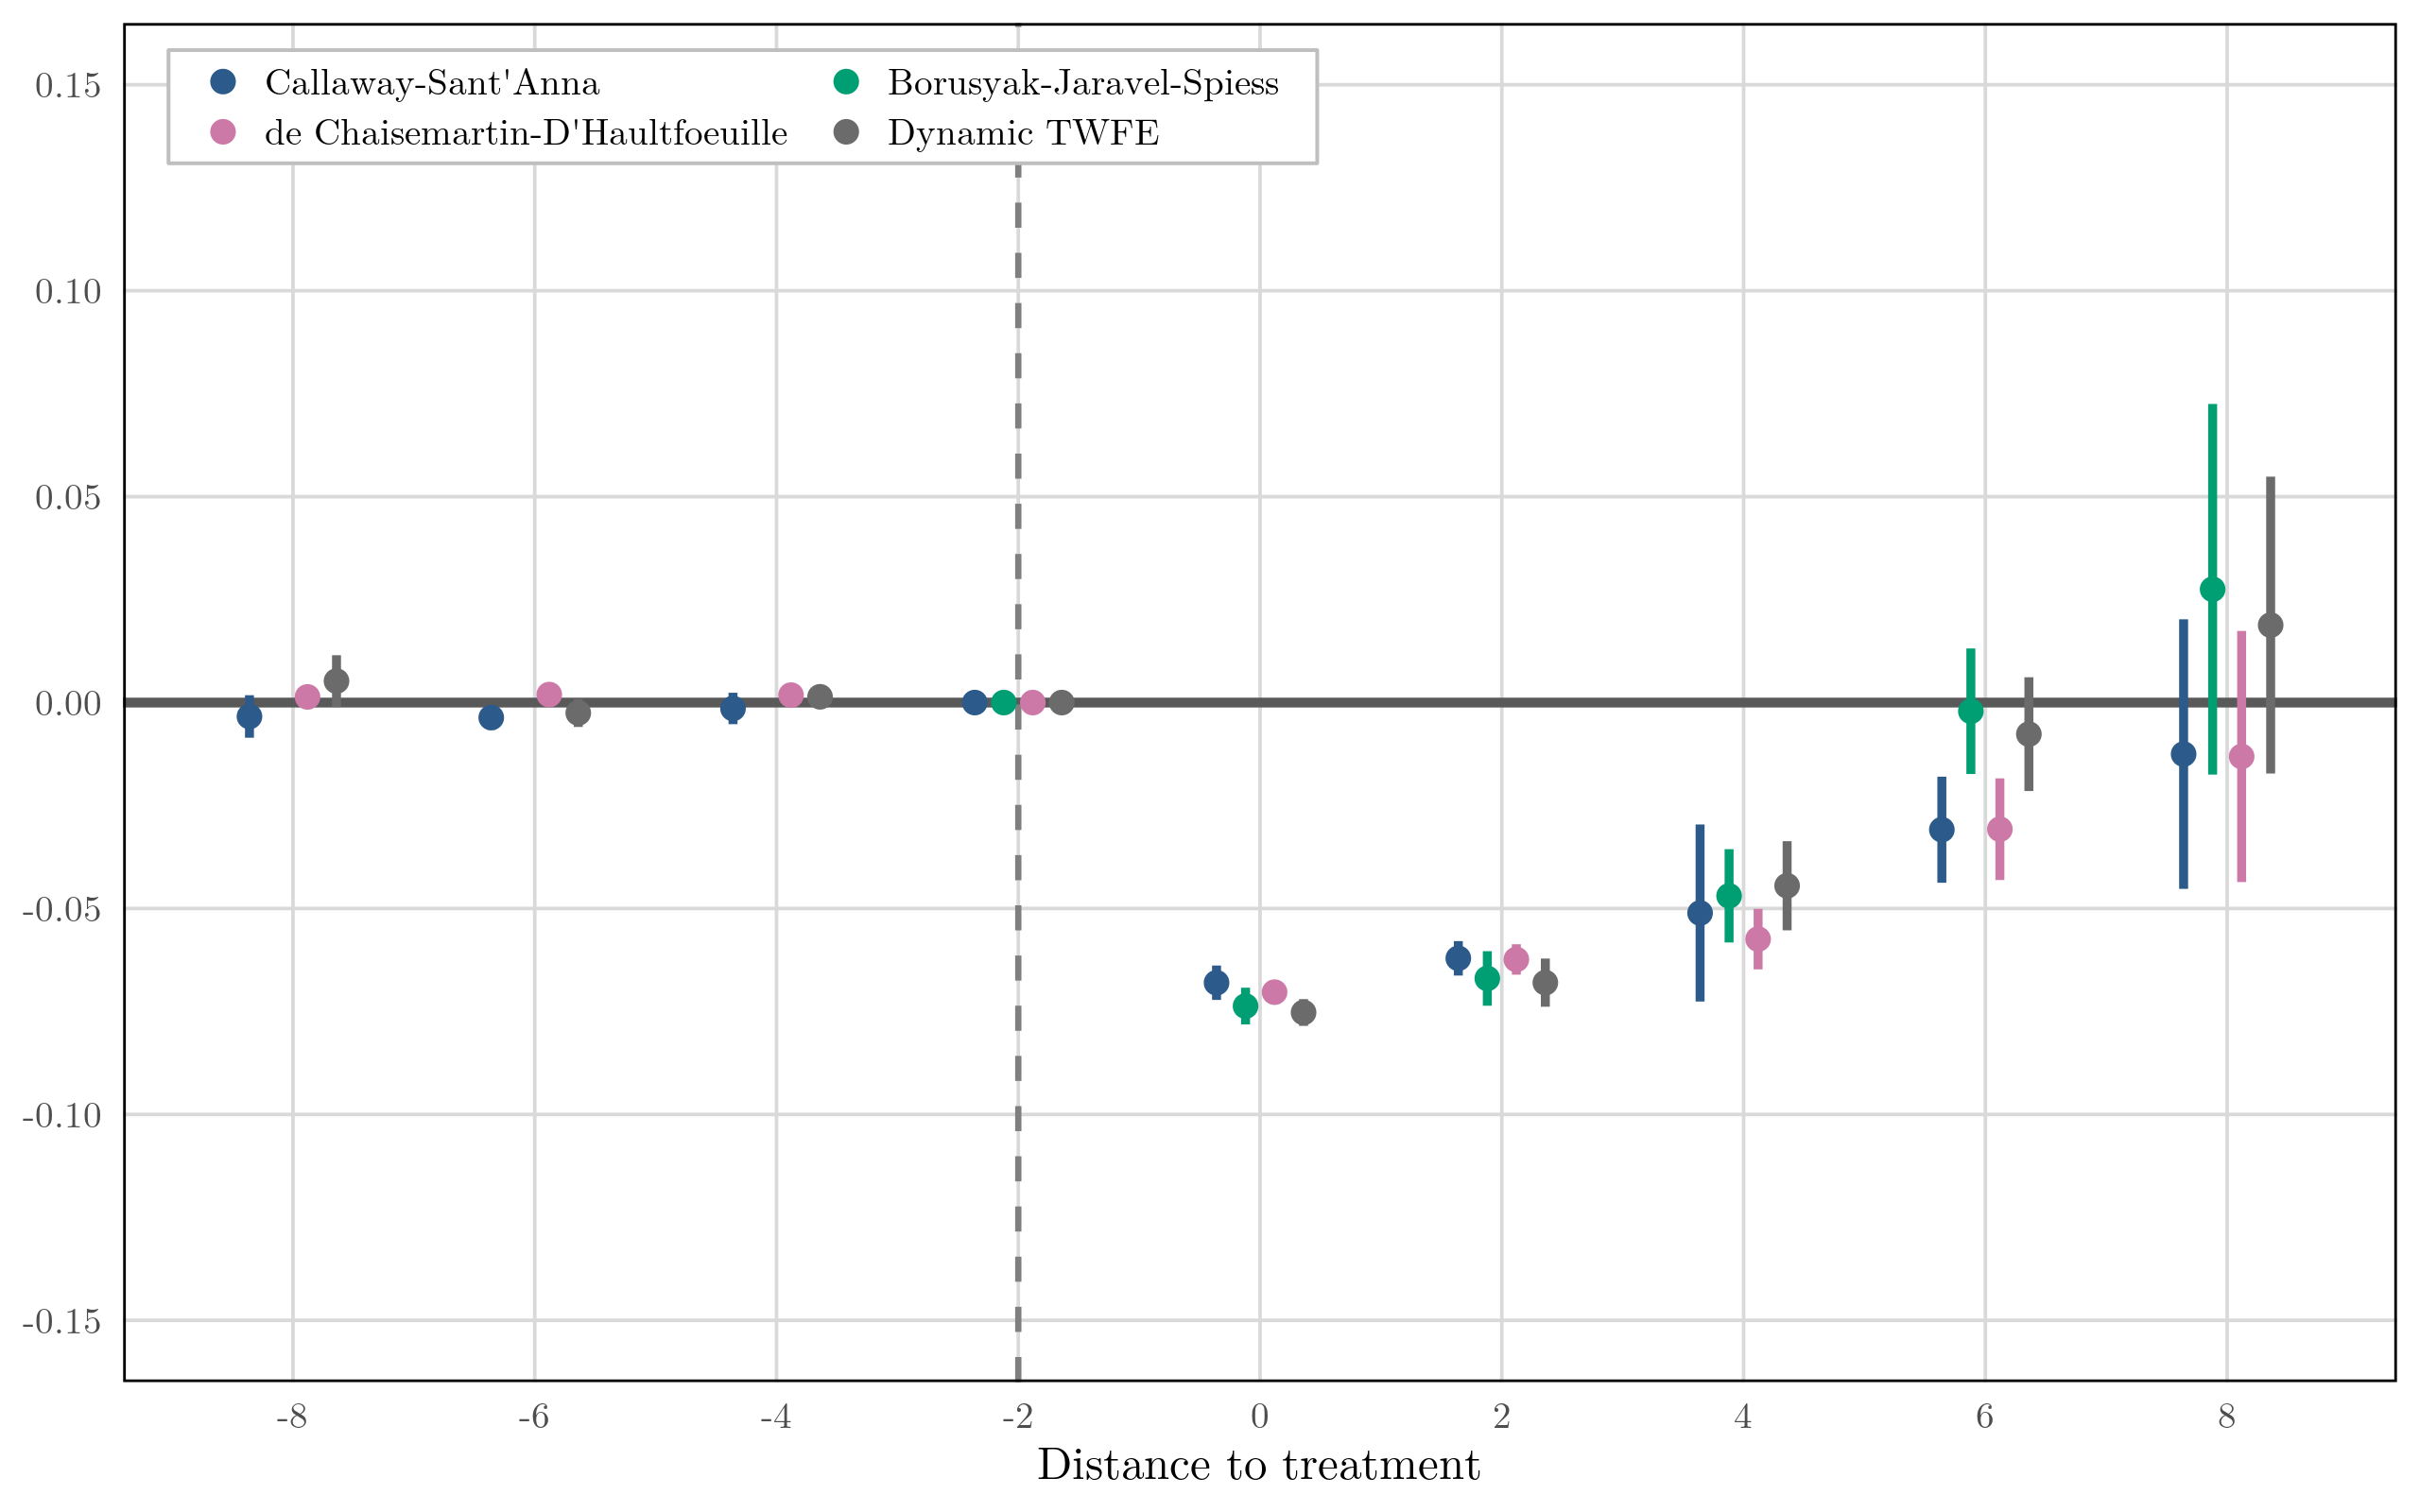
\includegraphics[width=0.72\textwidth]{../resources/regressions/bvr/log_num_voters/including_hybrid/other_estimators/estimator_comparison.png}
    \vspace{0.75em}
    \begin{minipage}{\textwidth}
        {\footnotesize \textbf{Note:} Each point reports an event-time estimate and each whisker a 95\% confidence interval for the hybrid-inclusive treatment definition. Colors identify the estimator. The Callaway--Sant'Anna series uses never-treated municipalities as the control group; the comparison series report dynamic TWFE, Borusyak--Jaravel--Spiess, and de Chaisemartin--D'Haultfoeuille alternatives. \par}
    \end{minipage}
\end{figure}

\begin{figure}[p]
    \caption{Including Hybrid Municipalities: Education Composition Across Estimators}
    \label{fig:appendix-composition-including-hybrid-estimator-comparison}
    \centering
    \begin{subfigure}[b]{0.49\textwidth}
        \centering
        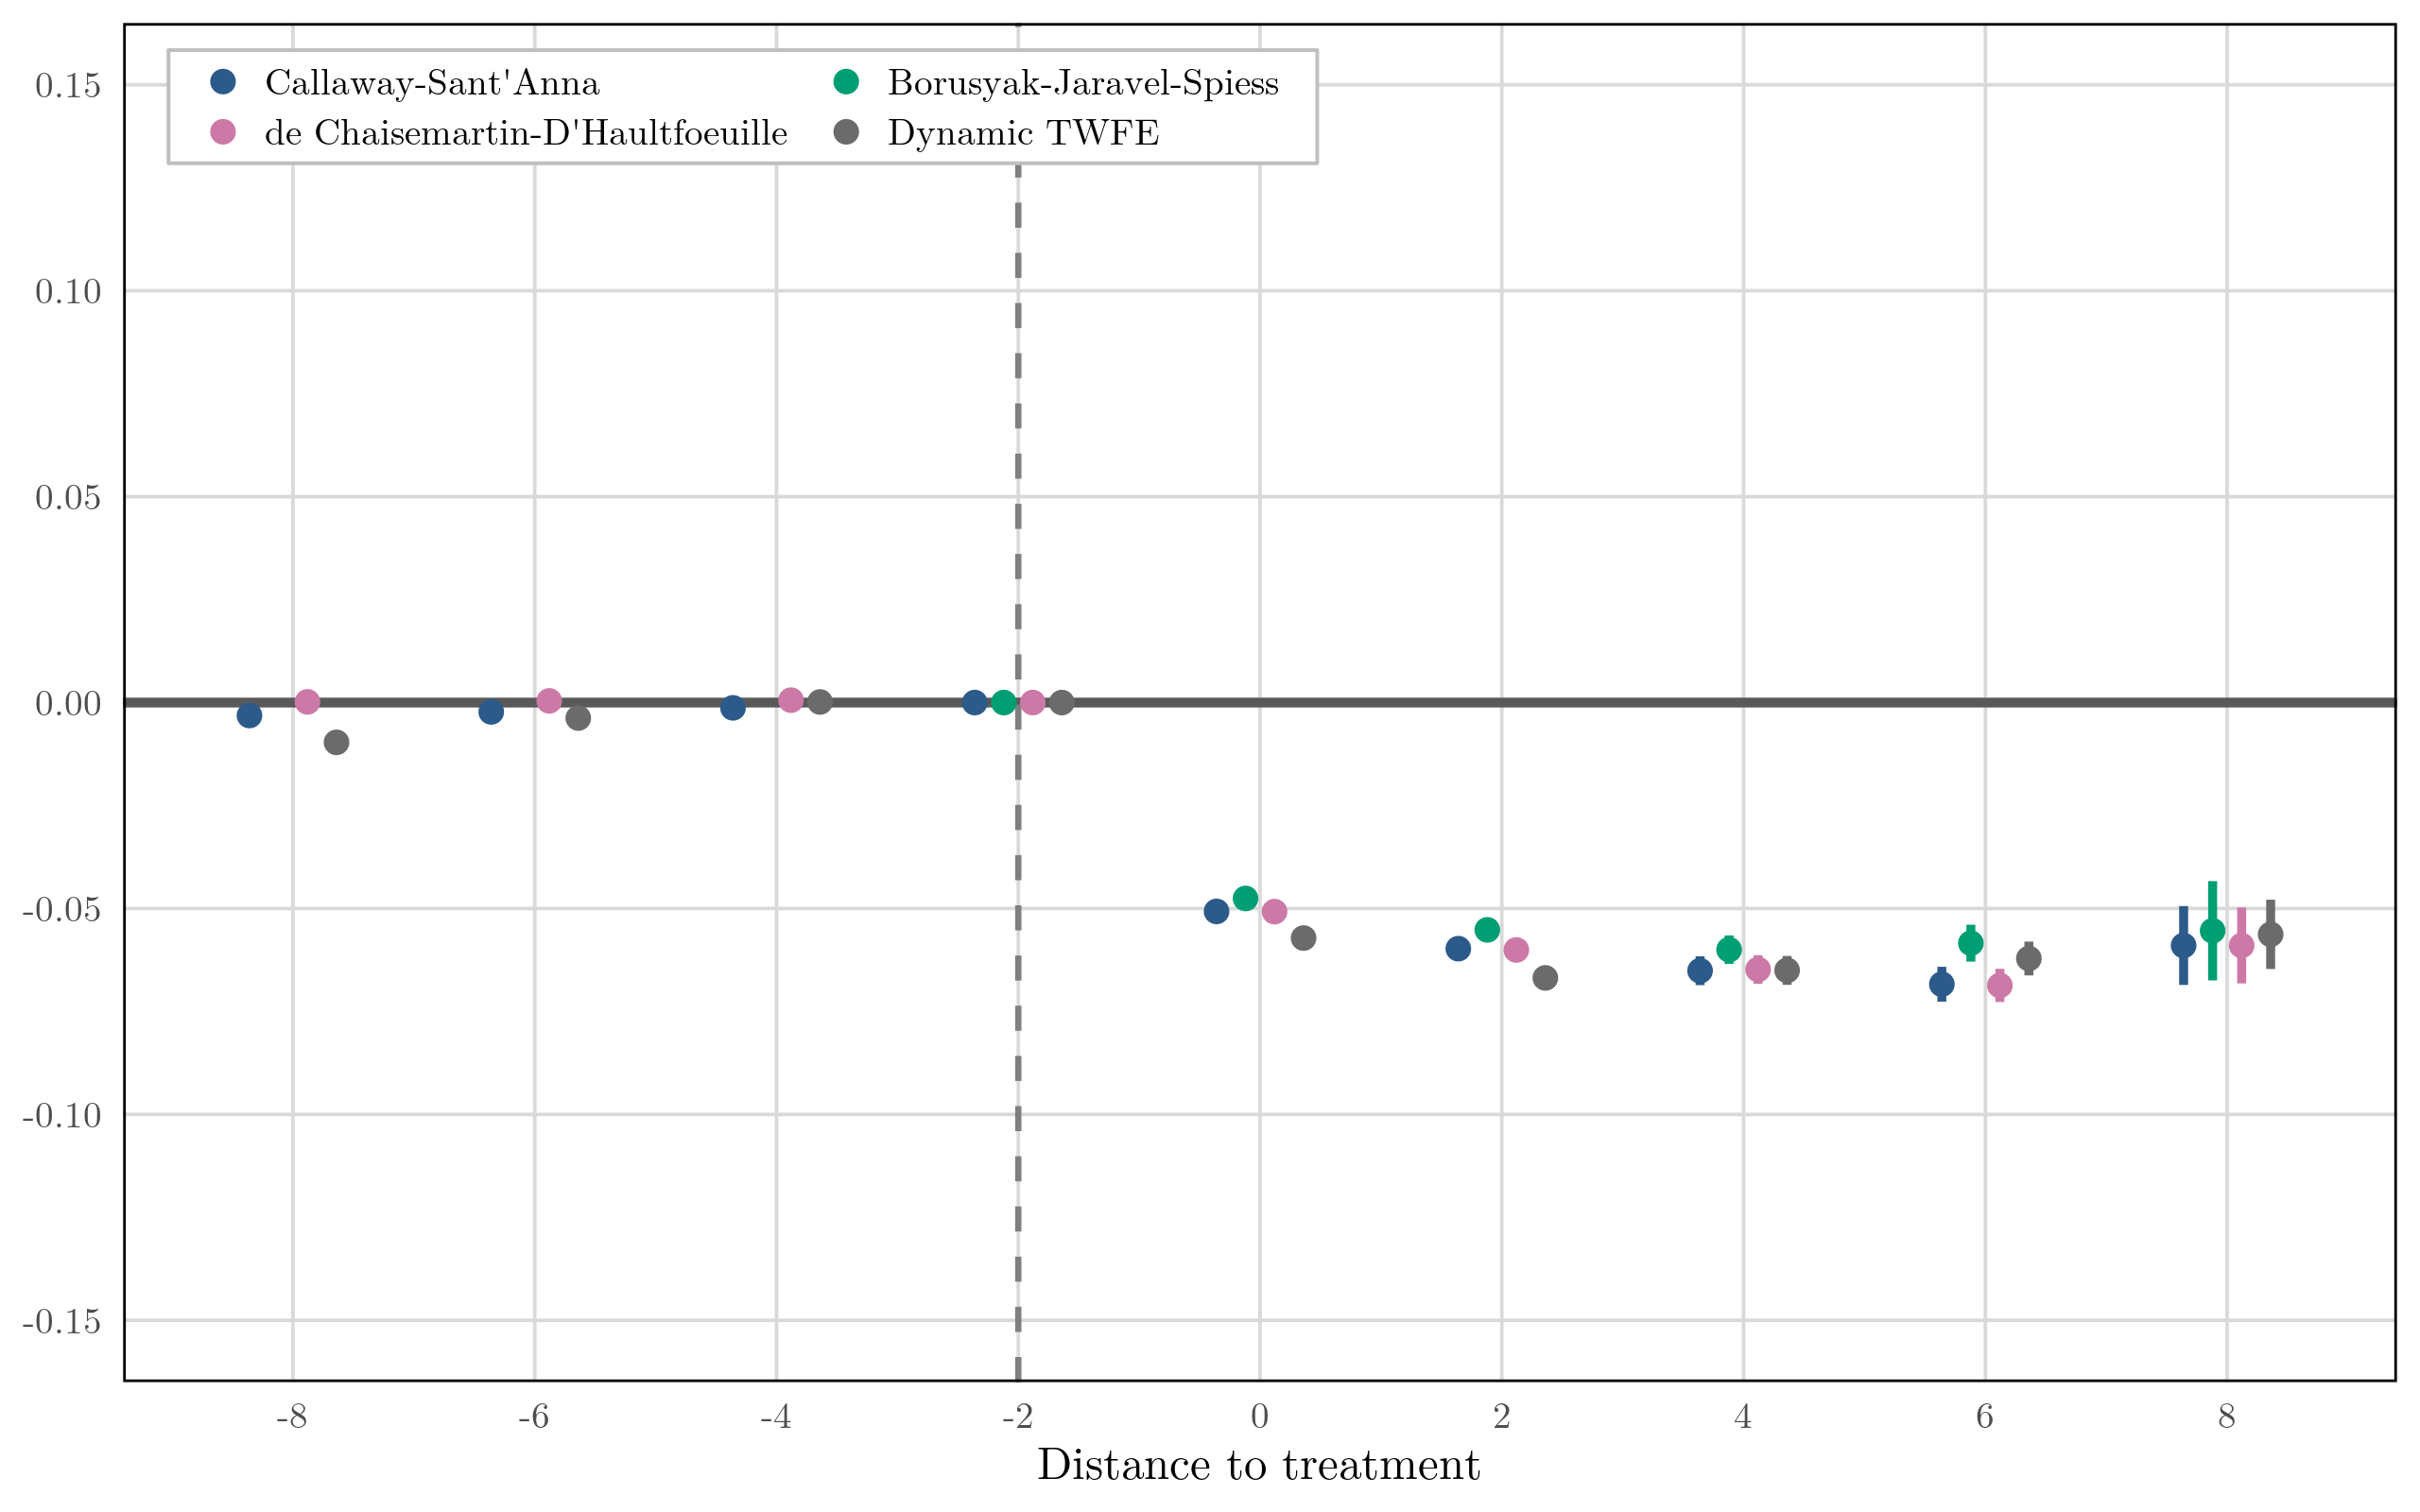
\includegraphics[width=\textwidth]{../resources/regressions/bvr/pct_voters_low_ed/including_hybrid/other_estimators/estimator_comparison.png}
        \caption{Low-education share}
        \label{fig:appendix-low-education-including-hybrid-estimator-comparison}
    \end{subfigure}
    \hfill
    \begin{subfigure}[b]{0.49\textwidth}
        \centering
        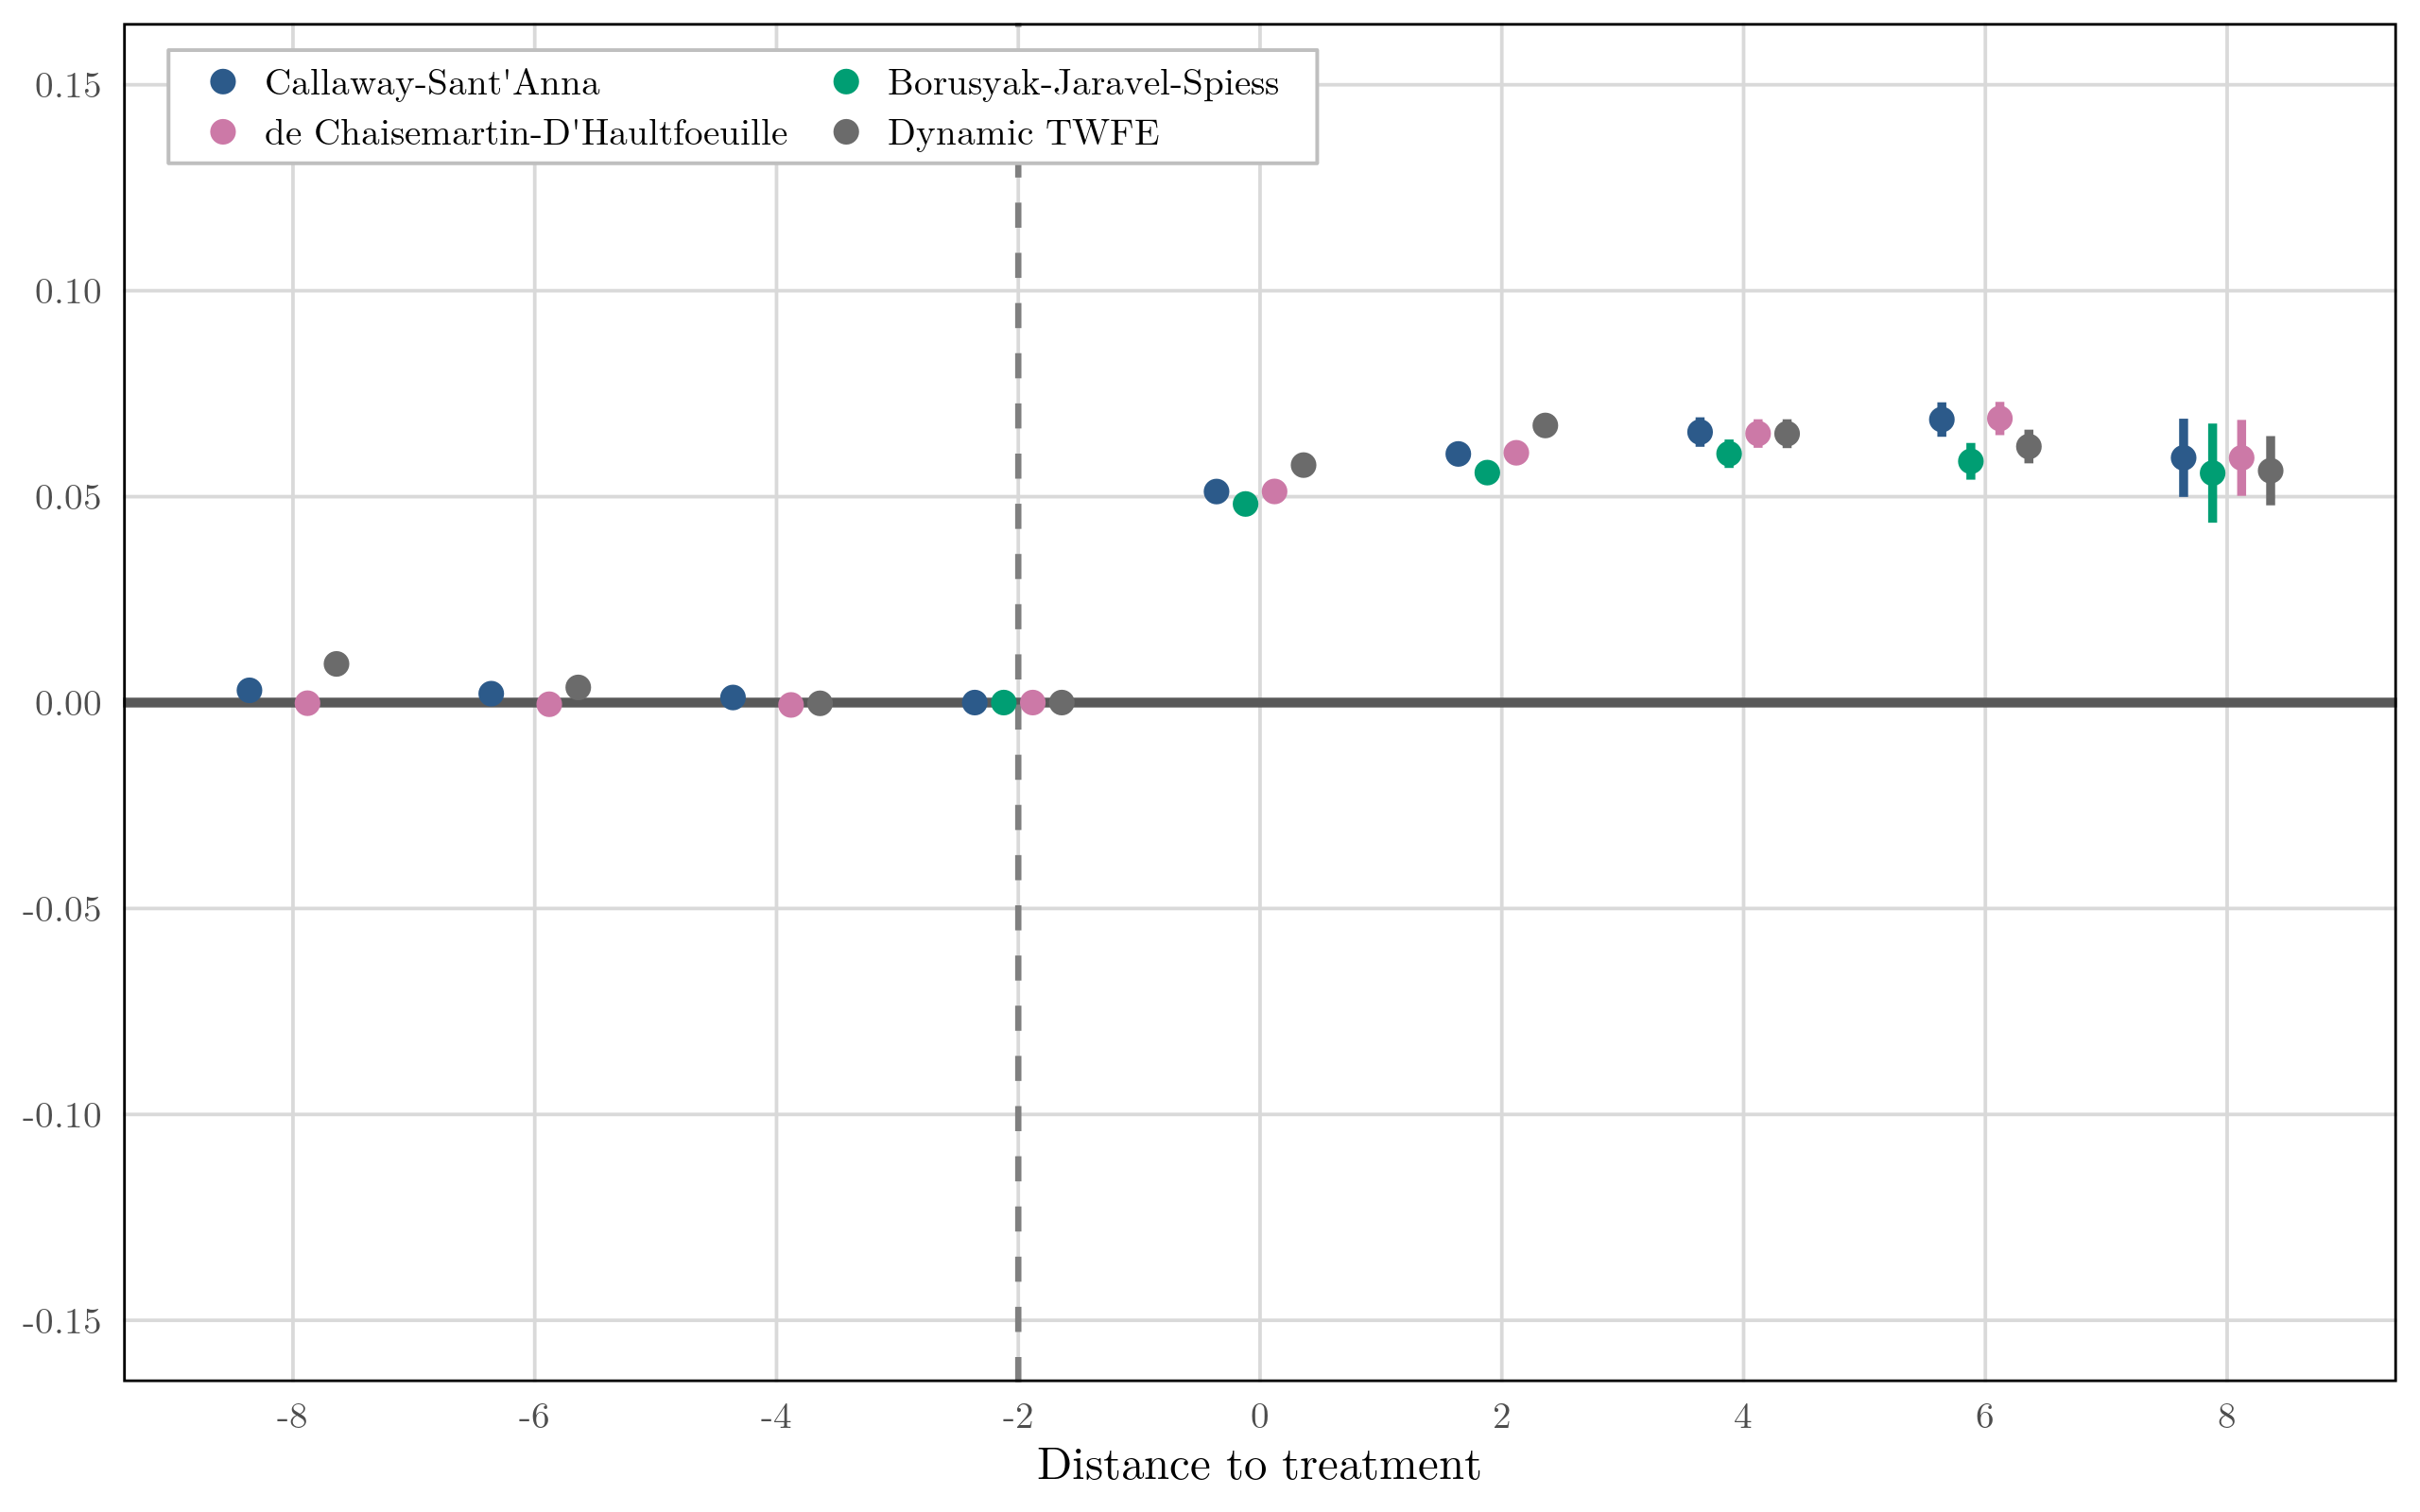
\includegraphics[width=\textwidth]{../resources/regressions/bvr/pct_voters_high_ed/including_hybrid/other_estimators/estimator_comparison.png}
        \caption{High-education share}
        \label{fig:appendix-high-education-including-hybrid-estimator-comparison}
    \end{subfigure}
    \vspace{0.75em}
    \begin{minipage}{\textwidth}
        {\footnotesize \textbf{Note:} Each point reports an event-time estimate and each whisker a 95\% confidence interval for the hybrid-inclusive treatment definition. Colors identify the estimator. Panel (a) uses the share of registered voters with schooling below completed secondary education as the outcome. Panel (b) uses the share with incomplete secondary schooling or more. \par}
    \end{minipage}
\end{figure}
